\documentclass{article}
\usepackage{graphicx} 
\usepackage[utf8]{inputenc}
\usepackage{amsmath, amsfonts, amssymb, bm}
\usepackage{graphicx, geometry, wrapfig, float, multicol, mathtools, array, csquotes, lscape, setspace}
\usepackage[dvipsnames]{xcolor}
\usepackage[export]{adjustbox}
\usepackage{tikz}
\usepackage[most]{tcolorbox}
\usetikzlibrary{positioning, fit}
\usepackage{multirow, booktabs, makecell, diagbox}
\usepackage{soul}
\usepackage{hyperref}
\usepackage{xstring}

\hypersetup{
    colorlinks=true,
    allcolors=.,
    pdftitle={Reinforcement Learning Notes},
    linkcolor=black
    }
\geometry{
    top=3.5cm,
    bottom=3.0cm,
    outer=2.0cm,
    inner=3.0cm
}
% Required for inserting images
\setlength{\parindent}{0mm}
\DeclareMathOperator{\EX}{\mathbb{E}}% expected value
\newcommand{\HRule}[1]{\rule{\linewidth}{#1}}
\renewcommand{\ref}[1]{\textbf{\ref{#1}}}

\begin{document}
\title{ \normalsize \textsc{}
		\\ [2.0cm]
		\HRule{1.5pt} \\
		\LARGE \textbf{\uppercase{Reinforcement Learning}
		\HRule{2.0pt} \\ [0.6cm] \LARGE{Academic Year: 2022/2023} \vspace*{10\baselineskip}}
		}

\author{\textbf{Author} \\ 
    Lorenzo Bonanni\\
    lorenzo.bonanni@studenti.univr.it}




\maketitle
\newpage
\tableofcontents

\newcommand{\splittedtext}[2]{\begin{matrix}\mbox{\footnotesize#1}\\\mbox{\footnotesize#2}\end{matrix}}

\section{On-Policy Prediction with Approximation}
If we want to apply a Reinforcement Learning method to a large state space problem by using tabular methods it becomes infeasible.
For example if the state is represented by an image, the state space would be larger than the number of atoms in the universe.

That causes two main problems:

\begin{enumerate}
    \item \textbf{Memory} we would have to store in memory a table of the size of the state space times the number of actions.
    \item \textbf{Generalization} by having a huge space almost all states encountered have never been seen before so we would never converge our estimates.
\end{enumerate}

A possible solution to this problem is to combine RL with function approximation (i.e supervised learning).
This approach solves the previously described issues and transforms the problem from finding the optimal policy to finding a good approximate solution. 
Approximations are based on parameterized functions ($\hat{v}(s,w)\approx v_\pi(s)$) and typically the number of weights is much smaller than the number of states.
By changing one weight we change the estimated value of many states, this makes reinforcement learning more powerful but
also more difficult to manage and understand.

\subsection{Value-function approximation}
All prediction methods seen so far are based on updates of an
estimated value function.
\begin{itemize}
    \item \textbf{MC update}: $\underbrace{S_t}_{\splittedtext{State}{Updated}}\mapsto \underbrace{G_t}_{\splittedtext{Update}{Target}}$
    \item \textbf{TD update}:$\underbrace{S_t}_{\splittedtext{State}{Updated}}\mapsto \underbrace{R_{t+1}+\gamma\hat{v}(S_{t+1}, w_t)}_{\splittedtext{Update}{Target}}$
    \item \textbf{DP update}:$\underbrace{S_t}_{\splittedtext{State}{Updated}}\mapsto \underbrace{\EX{[R_{t+1}+\gamma\hat{v}(S_{t+1}, w_t)\;|\;S_t=s]}}_{\splittedtext{Update}{Target}}$
\end{itemize}

We can use the current target as the y to predict. Not all function approximation are equally well suited.\\

For a function to be good it needs to:
\begin{itemize}
    \item learn from incrementally obtained data
    \item deal with non-stationary reward functions
\end{itemize}
\subsection{The Prediction Objective}
In tabular case a continuous measure of prediction quality was not necessary because the learned value function could become equal to the true one and updates affect only single states.
With function approximation these two assumptions are not guaranteed.\\

We define which states we care most about defining a state distribution $\mu(s)\ge0,\sum_s\mu(s)=1$.

Then a natural objective function is the \textbf{Mean Squared Value Error}
\begin{align}
    \overline{\mbox{VE}}(w)\doteq\sum_{s\in\mathcal{S}}\mu(s)[v_\pi(s)-\hat{v}(s, w)]^2
\end{align}

Often $\mu(s)$ is set to the fraction of time spent in state s (\textbf{on-policy
distribution}).
In episodic tasks: let $h(s)$ the probability an episode starts in state $s$,
then the number of time steps spent, on average, in state $s$ in a
single episode is:

\begin{align}
    \eta(s)=h(s)+\sum_{\bar{s}}\eta(\bar{s})\sum_a\pi(a | \bar{s})p(s | \bar{s},a),\quad\forall s\in S
\end{align}
\begin{align}
    \mu(s)=\frac{\eta(s)}{\sum_{s'}\eta(s')}\quad\forall s\in S
\end{align}

In continuing tasks the on-policy distribution is the stationary
distribution under $\pi$. In episodic tasks it also depends on state initial
probability.\\


The goal of $\overline{\mbox{VE}}$ is to find a global optimum, namely a weight vector w* such that
\begin{align}
    \overline{\mbox{VE}}(w^*)\leq \overline{\mbox{VE}}(w)\quad \forall w\in W
\end{align}
For simple tasks(e.g., linear
models) is possible to achieve global optima but for complex ones(e.g., ANNs and decision trees) it is not always possible,there learning usually converges to local optima.
\subsection{Stochastic-Gradient and Semi-Gradient Methods}
Stochastic-Gradient methods are a class of learning methods for function approximation in value
prediction based on Stochastic Gradient Descent (SGD).\\

Before we start a bit of notation:
\begin{itemize}
    \item $\mathbf{w}\doteq(w_1,w_2,\dots,w_d)^T$ a weight vector
    \item $\hat{v}(s, w)$ is a differentiable function of w for all states s
\end{itemize}
At each time step $0,1,2,3,\dots$ we observe a new example $S_t\mapsto v_\pi(S_t)$ and update $\mathbf{w}_t$.\\

The goal of SGD is to minimize error on the observed examples it does so by adjusting $w$ after each example by a small amount in the direction that would most reduce the error on that example.
\begin{align}
    \mathbf{w}_{t+1}&\doteq \mathbf{w}_{t}-\frac{1}{2}\alpha\nabla[\underbrace{v_\pi(S_t)-\hat{v}(S_t, \mathbf{w}_{t})}_{Value\;Error}]^2 \\
    &=\mathbf{w}_{t}+\alpha[v_\pi(S_t)-\hat{v}(S_t, \mathbf{w}_{t})]\nabla \hat{v}(S_t, \mathbf{w}_{t})
    \label{eq:1}
\end{align}
where $\alpha>0$ is the learning rate and $\nabla f(\mathbf{w})\doteq\left(\frac{\partial f(\mathbf{w})}{\partial w_1}, \frac{\partial f(\mathbf{w})}{\partial w_2}), \dots, \frac{\partial f(\mathbf{w})}{\partial w_d}\right)^T$ gradient of f.

The negative gradient is the direction in which the error falls most rapidly.\\

Why performing only “small” steps? If we completely corrected each example in one step then we would not balance the error (which cannot be completely removed) on all samples.
Convergence results on SGD assume that $\alpha$ decreses over time according to the following conditions:
\begin{align*}
    \sum^\infty_{n=1}\alpha_n=\infty\quad and \quad \sum^\infty_{n=1}\alpha^2_n<\infty
\end{align*}
\begin{itemize}
    \item \textbf{First condition:} guarantees that the steps are large enough to eventually overcome any initial condition or random fluctuations.
    \item \textbf{Second condition:} guarantees that eventually the steps become small enough to assure convergence
\end{itemize}
The problem with \ref{eq:1} is that $v_\pi(S_t)$ is unknown.

In practice the \textbf{target output observed} at time $t$, $U_t\in\mathbb{R}$ is \textbf{not the true value} $v_\pi(S_t)$ but some random approximation of it (e.g, noisy corrupted value of $v_\pi(S_t)$ or a bootstrapping target) so we'll perform an approximate update:
\begin{align}
    \mathbf{w}_{t+1}\doteq\mathbf{w}_{t}+\alpha[U_t-\hat{v}(S_t, \mathbf{w}_{t})]\nabla \hat{v}(S_t, \mathbf{w}_{t})
\end{align}
If $U_t$ is an unbiased estimate of the value, i.e $\mathbb{E}[U_t|S_t=s]=v_\pi(S_t)$ then $\mathbf{w}_t$ is guaranteed to converge to local optimum.\\

The \textbf{Monte Carlo target} $U_t\doteq G_t$ is an unbiased estimate of $v_\pi(S_t)$, hence the SGD version of MC state-value prediction converges.\\

\begin{tcolorbox}[colback=black!7!white,colframe=black!75!white,title=\textbf{Gradient Monte Carlo Algorithm for Estimating} $\mathbf{\hat{v}\approx v_\pi}$]
Input: the policy $\pi$ to be evaluated\\
Input: a differentiable function $\hat{v}: \mathcal{S}\times\mathbb{R}^d\rightarrow\mathbb{R}$\\
Algorithm parameter: step size $\alpha > 0$\\
Initialize value-function weights $\mathbf{w}\in\mathbb{R}^d$ arbitrarily (e.g., $\mathbf{w=0}$)\\

Loop forever (for each episode):

    \qquad Generate an episode $S_0, A_0, R_1, S_1, A_1,\dots,R_T,S_T$ using $\pi$

    \qquad Loop for each step of episode, $t=0,1,\dots, T-1$:

    \qquad\qquad $G\leftarrow \gamma G+R_{t+1}$

    \qquad\qquad $\mathbf{w}\leftarrow\mathbf{w}+\alpha[G_t-\hat{v}(S_t, \mathbf{w})]\nabla \hat{v}(S_t, \mathbf{w})$
\end{tcolorbox}

MC provides a non bootstrapping estimate of $v_\pi$. If a bootstrapping estimate is used as target then the convergence is not guaranteed, this because they depend on the current value of the
weight vector $w_t$, which implies that they will be biased and that they will not produce a true gradient-descent method.\\

Hence those methods are called semi-gradient methods since they take into account the effect of changing the weight vector $w_t$ on the estimate, but ignore its effect on the target, that means that they include only a part of the gradient. Although semi-gradient (bootstrapping) methods do not converge as robustly as gradient methods, they do converge reliably in important cases such as the linear case. Moreover, they offer important advantages that make them
often clearly preferred. One reason for this is that they typically enable significantly faster learning. Another is that they enable learning to be continual and online, without waiting for the end of an episode.
\begin{tcolorbox}[colback=black!7!white,colframe=black!75!white,title=\textbf{Semi-gradient TD(0) for Estimating} $\mathbf{\hat{v}\approx v_\pi}$]
Input: the policy $\pi$ to be evaluated\\
Input: a differentiable function $\hat{v}: \mathcal{S}^+\times\mathbb{R}^d\rightarrow\mathbb{R}$\\
Algorithm parameter: step size $\alpha > 0$\\
Initialize value-function weights $\mathbf{w}\in\mathbb{R}^d$ arbitrarily (e.g., $\mathbf{w=0}$)\\

Loop for each episode:

    \qquad Initialize S

    \qquad Loop for each step of episode:

    \qquad\qquad Choose $A\sim\pi(\cdot|S)$

    \qquad\qquad Take action A, observe R, S'

    \qquad\qquad $\mathbf{w}\leftarrow\mathbf{w}+\alpha[R+\gamma\hat{v}(S', \mathbf{w})-\hat{v}(S, \mathbf{w})]\nabla \hat{v}(S, \mathbf{w})$

    \qquad\qquad $S\leftarrow S'$

    \qquad until S is terminal
\end{tcolorbox}

\subsection{Linear Value Function Approximation}
One of the most important special cases of function approximation is that in which the approximate function, $\hat{v}(\cdot,\mathbf{w})$, is a linear function of the weight vector, \textbf{w}. Corresponding to every state s, there is a real-valued feature vector $\mathbf{x}(s)\doteq (x_1(s), x_2(s), \dots, x_d(s))^T$ with the same number of components as \textbf{w}. Linear methods approximate state-value function by the inner product between \textbf{w} and \textbf{x}(s):
\begin{align}
    \hat{v}(s,\mathbf{w})\doteq \mathbf{w}^T\mathbf{x}(s)\doteq\sum_{i=1}^d w_i x_i(s)
\end{align}
In this case the approximate value function is said to be \textit{linear in the weights}, or simply \textit{linear}.

It is natural to use SGD updates with linear function approximation. The gradient of the approximate value function with respect to $w$ in this case is
\begin{align}
    \nabla\hat{v}(s,\mathbf{w})&=\mathbf{x}(s)\\
\end{align}
Hence the SGD update becomes:
\begin{align}
    \mathbf{w}_{t+1}\doteq\mathbf{w}_{t}+\alpha&[U_t-\hat{v}(S_t, \mathbf{w}_{t})]\mathbf{x}(s)
\end{align}
Because it is so simple, the linear SGD case is one of the most favorable for mathematical analysis. Almost all useful convergence results for learning systems of all kinds are for linear (or simpler) function approximation methods.
In particular, in the linear case there is only one optimum, and thus any method that is \textbf{guaranteed to converge} to a local optimum is automatically guaranteed to converge to the global optimum. Other advantages include data efficiency and computational efficiency.\\

For example, the Gradient Monte Carlo algorithm converges to the global optimum of the $\overline{VE}$ under a linear function approximation if $\alpha$ is reduced over time according to the usual conditions. The semi-gradient TD(0) algorithm also converges under linear function approximation. This result requires a separate theorem (the weight vector converges to a point near the local optimum).

The update at each time $t$ is:
\begin{align}
    \mathbf{w}_{t+1}&\doteq\mathbf{w}_t+\alpha\left(R_{t+1}+\gamma\mathbf{w}_t^T\mathbf{x}_{t+1}-\mathbf{w}_t^T\mathbf{x}_t\right)\mathbf{x}_t\\
    &=\mathbf{w}_t+\alpha\left(R_{t+1}\mathbf{x}_t-\mathbf{x}_t(\mathbf{x}_t-\gamma\mathbf{x}_{t+1})^T\mathbf{w}_t\right)
\end{align}

\subsection{Feature Constructions for Linear Methods}
Linear methods are interesting because of their \textbf{convergence guarantees}, but also because in practice they can be very \textbf{efficient} in terms of both \textbf{data} and \textbf{computation}.
Whether or not this is so \textbf{depends critically} on how the \textbf{states} are \textbf{represented} in terms of features. Choosing features appropriate to the task is an important way of adding prior domain knowledge to reinforcement learning systems. Intuitively, the features should correspond to the aspects of the state space along which generalization may be appropriate. If we are valuing geometric objects, for example, we might want to have features for each possible shape, color, size, or function. If we are valuing states of a mobile robot, then we might want to have features for locations, degrees of remaining battery power, recent sonar readings, and so on. One of the main limitations of linear approximation is that it cannot consider interactions between features for example in the pole-balancing task, high angular velocity can be either good or bed depending on the angle.
A \textbf{linear} value \textbf{function cannot represent} this if this \textbf{features} are \textbf{coded separately} for the angle and the angular velocity

\subsection{Nonlinear Value Function Approximation}
There exist several non-linear methods for approximating the value
function, such as:
\begin{itemize}
    \item Artificial Neural networks (ANNs)
    \item Memory-based (nonparametric) functions
    \item Kernel-based functions
\end{itemize}
ANNs have recently become the most popular approximation functions thanks to the fact that they are universal function approximators and that in deep architectures they can generate hierarchical representations of features automatically.

\section{On-Policy Control with Approximation}
In this chapter we return to the control problem, now with parametric approximation of the action-value function:
\begin{align}
    \hat{q}(s,a,\mathbf{w})\approx q_*(s,a)
\end{align}
We continue to restrict our attention to the on-policy and episodic case.
\subsection{Episodic Semi-Gradient Control}
The extension of state-value function approximators $\hat{v}(s,\mathbf{w})$ to action-value function approximators $\hat{q}(s,a,\mathbf{w})$ is straightforward.\\

Whereas before we considered random training examples of the form $S_t\mapsto U_t$, now we consider examples of the form $S_t, A_t\mapsto U_t$. The update target $U_t$ can be any approximation of $q_\pi(S_t, A_t)$, including the usual backed-up values such as the full Monte Carlo return ($G_t$) or any
of the \textit{n}-step Sarsa returns.\\

The general gradient-descent update for action-value prediction is:
\begin{align}
    \mathbf{w}_{t+1}\doteq\mathbf{w}_t+\alpha[\textcolor{blue}{U_t}-\hat{q}(S_t, A_t, \mathbf{w}_t)]\nabla \hat{q}(S_t, A_t, \mathbf{w}_t)
\end{align}

For the one-step Sarsa method it is:
\begin{align}
    \mathbf{w}_{t+1}\doteq\mathbf{w}_t+\alpha[\textcolor{blue}{R_{t+1}+\gamma\hat{q}(S_{t+1}, A_{t+1}, \mathbf{w}_t)}-\hat{q}(S_t, A_t, \mathbf{w}_t)]\nabla \hat{q}(S_t, A_t, \mathbf{w}_t)
\end{align}
We call this method episodic semi-gradient one-step Sarsa.
To form control methods, we need to couple such action-value prediction methods with techniques for policy improvement and action selection. If the action set is discrete and not too large, then we can use the techniques already developed in previous chapters. That is, for each possible action $A$ available in the current state $S_t$, we can compute $q(S_t, A_t, \mathbf{w}_t)$ and then find the greedy action $A_t^*=arg\max_a \hat{q}(S_t, A_t, \mathbf{w}_t)$.

Policy improvement is then performed by changing the estimation policy to a soft-approximation of the greedy policy, e.g., the $\varepsilon$-greedy policy.

\begin{tcolorbox}[colback=black!7!white,colframe=black!75!white,title=\textbf{Episodic Semi-gradient Sarsa for Estimating} $\mathbf{\hat{q}\approx q_\pi}$]
Input: a differentiable action-value function parameterization $\hat{q}: \mathcal{S}\times\mathcal{A}\times\mathbb{R}^d\rightarrow\mathbb{R}$\\
Algorithm parameter: step size $\alpha > 0$, small $\varepsilon > 0$\\
Initialize value-function weights $\mathbf{w}\in\mathbb{R}^d$ arbitrarily (e.g., $\mathbf{w=0}$)\\

Loop for each episode:

    \qquad Initialize S, A $\leftarrow$ initial state and action of episode (e.g., $\varepsilon$-greedy)

    \qquad Loop for each step of episode:

    \qquad\qquad Take action A, observe R, S'

    \qquad\qquad If S' is terminal:

        \qquad\qquad\qquad $\mathbf{w}\leftarrow\mathbf{w}+\alpha[R-\hat{q}(S, A, \mathbf{w})]\nabla \hat{q}(S, A, \mathbf{w})$

        \qquad\qquad\qquad Go to next episode

    \qquad\qquad Choose A' as a function of $\hat{q}(S', \cdot, \mathbf{w})$ (e.g., $\varepsilon$-greedy)

    \qquad\qquad $\mathbf{w}\leftarrow\mathbf{w}+\alpha[R+\gamma\hat{q}(S', A', \mathbf{w})-\hat{q}(S, A, \mathbf{w})]\nabla \hat{q}(S, A, \mathbf{w})$
    
    \qquad\qquad $S\leftarrow S'$

    \qquad\qquad $A\leftarrow A'$

\end{tcolorbox}

\subsection{Deep Q Networks}
The basic idea of Deep Q Networks to use deep neural networks as a non-linear function approximator for the action value function in a semi-gradient form of Q-learning.

The input of the Q network is the current state and the output is the estimated optimal action values for the input state.

The semi-gradient form of Q-learning used by DQN to update the network’s weight is
\begin{align}
    \mathbf{w}_{t+1}=\mathbf{w}_t+\alpha[\underbrace{R_{t+1}+\gamma\max_a\hat{q}(S_{t+1}, a, \mathbf{w}_t)}_{Target\;value}-\underbrace{\hat{q}(S_t, A_t, \mathbf{w}_t)}_{Action\;value}]\nabla \hat{q}(S_t, A_t, \mathbf{w}_t)
\end{align}
The problem with this is RL is unstable or even deverges with nonlinear function approximators (e.g., ANNs) of the action-value function (Minh et al., 2015).
This is caused mainly by three things:
\begin{enumerate}
    \item \textbf{Correlations in the sequence of observations}: most deep learning algorithms assume the data samples to be independent, while in reinforcement learning one typically encounters sequences of highly correlated states. 
    \item Small updates to q may significantly change the policy and change data distribution
    \item Correlation between action-values $\hat{q}(S_t, A_t, \mathbf{w}_t)$ and target values $R_{t+1}+\gamma\max_a\hat{q}(S_{t+1}, A_{t+1}, \mathbf{w}_t)$
\end{enumerate}
The solutions to those problems are:
\begin{enumerate}
    \item A biologically inspired mechanism for \textbf{experience replay}
    \item The usage of \textbf{two separate networks} to estimate action values in the Q-network and the target value
\end{enumerate}
\subsubsection{Experience Replay}
The idea is to store agent experience in a replay memory then used to perform weight updates. After each step a tuple $(S_t, A_t, R_{t+1}, S_{t+1})$ is added to the replay memory. This experience is accumulated over many episodes. At each step  multiple Q-learning \textbf{updates} (a mini-batch) are performed based on experience \textbf{sampled} uniformly at \textbf{random} from the replay memory.
This has two main advantages:
\begin{enumerate}
    \item Reduced variance of weight update (reduces cause 2)
    \item The correlation in the sequences of observations is eliminated and hence one source instability is removed (reduces cause 1)
\end{enumerate}
When learning on-policy the current parameters determine the next data sample that the parameters are trained on. For example, if the maximizing action is to move left then the training samples will be dominated by samples from the left-hand side; if the maximizing action then switches to the right then the training distribution will also switch. It is easy to see how unwanted feedback loops may arise and the parameters could get stuck in a poor local minimum, or even diverge catastrophically. By using experience replay the behavior distribution is averaged over many of its previous states, smoothing out learning and avoiding oscillations or divergence in the parameters

\subsubsection{Double DQN}
Two networks are used. One for estimating action values, another for estimating target values.
The new update rule is:
\begin{align}
    \mathbf{w}_{t+1}=\mathbf{w}_t+\alpha[R_{t+1}+\gamma\max_a\underbrace{\colorbox{red!60!white}{$\Tilde{q}(S_{t+1}, a, \mathbf{w}_t)$}}_{ANN\;2}-\underbrace{\colorbox{lime}{$\hat{q}(S_t, A_t, \mathbf{w}_t$})}_{ANN\;1}]\nabla \underbrace{\colorbox{lime}{$\hat{q}(S_t, A_t, \mathbf{w}_t)$}}_{ANN\;1}
\end{align}
After C updates of the weights w of the action-value network (ANN 1) these weights are copied to the second network (ANN 2) used to compute the target values. By doing so we are improving stability and reducing cause 3.
\section{Policy Gradient Methods}
So far, all the methods we have discussed are action-value methods. These methods estimate action values and use them to select actions, but they do not explicitly represent the policy function.\\

In contrast, {policy gradient methods take a different approach. They learn a parameterized policy function $\pi(a|s, \theta)$and use this function to select actions without relying on value functions. Although a value function can still be used to learn the policy parameter $\bm{\theta}$, it is not necessary for action selection.

Actor Critic methods are a type of policy gradient methods that also approximate the value function. They consist of two main components:
\begin{itemize}
    \item Actor: learn policy function
    \item Critic: learn value function
\end{itemize}

Before we proceed, let's introduce some notation:
\begin{itemize}
    \item The policy's parameter vector is denoted as $\bm{\theta}\in\mathbb{R}^{d'}$.
    \item $\pi(a|s, \bm{\theta})$ represents the probability of selecting action $a$ given state $s$ and policy parameters $\bm{\theta}$. In other words, $\pi(a|s, \bm{\theta})=Pr\{A_t=a|S_t=s,\bm{\theta}_t=\bm{\theta}\}$.
    \item If the method requires it, the learned value function is denoted as $\hat{v}(s, \bm{w})$ and it has parameters $\bm{w}\in\mathbb{R}^{d}$.
    \item $J(\bm{\theta})$ denotes a measure of policy performance, which depends on the policy parameters."
\end{itemize}

The objective of policy gradient methods is to find the optimal parameters $\bm{\theta}$ that maximize the performance measure $J(\bm{\theta})$.

The parameter updates in these methods can be approximated using gradient ascent, as follows:

\begin{align}
\bm{\theta}_{t+1} = \bm{\theta}_t + \alpha \widehat{\nabla J(\bm{\theta}_t})
\end{align}

Here, $\widehat{\nabla J(\bm{\theta}_t})\in \mathbb{R}^{d'}$ represents a stochastic estimate of the gradient of $J(\bm{\theta})$ with respect to $\bm{\theta}_t$. The learning rate is denoted by $\alpha$.\\

In the episodic case, the performance is measured by the value of the starting state under the parameterized policy. In contrast, in the continuing case, performance is assessed based on the average reward rate.

\subsection{Policy Approximation and its Advantages}
In policy gradient methods, the policy can be parameterized in any way as long as $\pi(a|s, \bm{\theta})$ is differentiable w.r.t its parameters. In practice to ensure exploration we require the policy never to become deterministic, (i.e that $\pi(a|s, \bm{\theta})\in(0,1)$).

If the action space is Discrete (and not too large) then a natural and common kind of parameterization is to form parameterized numerical preferences $h(s,a,\bm{\theta})\in\mathbb{R}$ for each state-action pair.
Probability is assigned to actions proportionally to preferences, e.g., according to exponential soft-max distribution(called soft-max in action preferences)
    \begin{align*}
         \pi(a|s, \bm{\theta})\doteq\frac{e^{h(s,a,\bm{\theta})}}{\sum_b e^{h(s,b,\bm{\theta})}}
    \end{align*}

Preferences can themselves be parameterized arbitrarily for example they might be computed by a deep ANN. In this case $\theta$ is a vector of connection weights or the preferences could be linear in the features: $h(s,a,\bm{\theta})=\bm{\theta}^T\bm{x}(s,a)$ with $\bm{x}(s,a)\in \mathbb{R}^{d'}$ features of the policy.

Action values could be used as preferences with soft-max but this would not allow the policy to approach deterministic behaviours. Instead, general action preferences do not have to approach specific values allowing them to approach also deterministic policies.

\subsection{Advantages of Policy Parametrization over Action Value Parametrization}
When comparing policy parametrization with action value parametrization, the former offers several advantages:

\begin{enumerate}
\item The policy function is often simpler and easier to approximate compared to the action-value function.
\item Policy parametrization allows for the incorporation of prior knowledge, which is a significant benefit and a common reason for choosing policy-based learning methods.
\item Unlike action-value methods, policy gradient methods (such as those employing soft-max in action preferences) facilitate the selection of actions with arbitrary probabilities, thus supporting the use of stochastic policies.
\item Policy-based methods can effectively handle continuous action spaces, whereas action-value methods may face challenges in such scenarios due to their inability to directly handle continuous actions.
\end{enumerate}

\subsection{The Policy Gradient Theorem}
In addition to the practical advantages of policy parameterization over $\varepsilon$-greedy action selection, there is also an important theoretical advantage. With continuous policy
parameterization the action probabilities change smoothly as a function of the learned
parameter, whereas in $\varepsilon$-greedy selection the action probabilities may change dramatically for an arbitrarily small change in the estimated action values.
Largely due to this characteristic, policy-gradient methods offer stronger convergence guarantees compared to action-value methods.\\

With function approximation, it may seem challenging to change the policy parameter in a way that ensures improvement. The problem is that \textbf{performance} depends on both the \textbf{action selections} and the \textbf{distribution of states} in which those selections are made, and that both of these are affected by the \textbf{policy parameter}. Given a state, the effect of the policy parameter on the actions, and thus on reward, can be computed in a relatively straightforward way from knowledge of the parameterization. But the effect of the policy on the state distribution is a function of the environment and is typically unknown. How can we estimate the performance gradient with respect to the policy parameter when the gradient depends on the unknown effect of policy changes on the state distribution?\\
\begin{center}
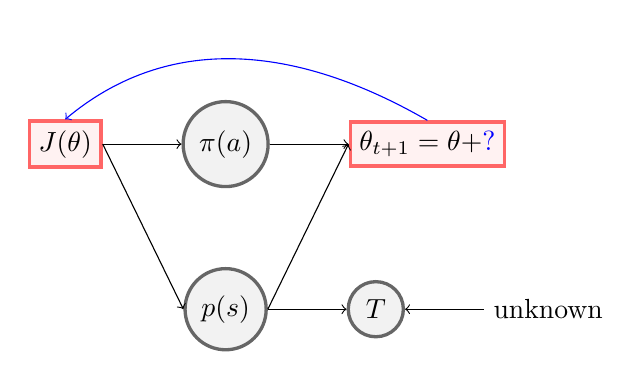
\begin{tikzpicture}[
roundnode/.style={circle, draw=black!60, fill=black!5, very thick, minimum size=7mm},
squarednode/.style={rectangle, draw=red!60, fill=red!5, very thick, minimum size=5mm},
]
    \node[squarednode]      (maintopic)                                                       {$J(\theta)$};
    \node[roundnode]        (rightcircle1)       [right=of maintopic]                         {$\pi(a)$};
    \node[roundnode]        (rightcircle2)       [right=of maintopic, below=of rightcircle1]  {$p(s)$};
    \node[roundnode]        (transition)         [right=of rightcircle2]                      {$T$};
    \node[squarednode]      (weights)            [right=of rightcircle1]                      {$\theta_{t+1}=\theta+\color{blue}?$};
    \node[]                 (text)               [right=of transition]                        {unknown};
    
    \draw[->] (maintopic.east)-- (rightcircle1.west);
    \draw[->] (maintopic.east) -- (rightcircle2.west);
    \draw[->] (rightcircle2.east) -- (transition.west);
    \draw[->] (rightcircle1.east) -- (weights.west);
    \draw[->] (rightcircle2.east) -- (weights.west);
    \draw[->, color=blue] (weights.north) to [out=150, in=40](maintopic.north);
    \draw[->] (text.west) -- (transition.east);
\end{tikzpicture}
\end{center}

\begin{tcolorbox}[colbacktitle=black!7!white,coltitle=black!75!white,title=\textbf{Proof of the Policy Gradient Theorem (episodic case)}]
With just elementary calculus and re-arranging of terms, we can prove the policy gradient theorem from first principles. To keep the notation simple, we leave it implicit in all cases that $\pi$ is a function of $\theta$, and all gradients are also implicitly with respect to $\theta$. First note that the gradient of the state-value function can be written in terms of the action-value function as
\begin{align*}
    \textcolor{blue}{\nabla v_\pi(s)}&=\nabla\Big[\sum_a\pi(a|s)q_\pi(s,a)\Big],\quad for\;all\;s\in S\\
    &=\sum_a\Big[\nabla\pi(a|s)q_\pi(s,a)+\pi(a|s)\nabla q_\pi(s,a)\Big]\\
    &=\sum_a\Big[\nabla\pi(a|s)q_\pi(s,a)+\pi(a|s)\nabla\sum_{s',r}p(s',r|s,a)(r+v_\pi(s') \Big]\\
    &=\sum_a\Bigg[\nabla\pi(a|s)q_\pi(s,a)+\pi(a|s)\sum_{s'}p(s'|s,a)\textcolor{blue}{\nabla v_\pi(s')} \Bigg]\\
    &=\sum_a\Bigg[\nabla\pi(a|s)q_\pi(s,a)+\pi(a|s)\sum_{s'}p(s'|s,a) \;\backslash \\
    &\quad\quad\textcolor{blue}{\sum_{a'}\Big[\nabla\pi(a'|s')q_\pi(s',a')+\pi(a'|s')\sum_{s''}p(s''|s',a')\nabla v_\pi(s'')\Big]}\Bigg]\\
    &=\sum_{x\in\mathcal{S}}\sum_{k=0}^{\infty} Pr(s\rightarrow x, k, \pi)\sum_a\nabla\pi(a|x)q_\pi(x,a)
\end{align*}
after repeated unrolling, where $Pr(s\rightarrow x, k, \pi)$ is the probability of transitioning
from state s to state $x$ in $k$ steps under policy $\pi$. It is then immediate that
\begin{align*}
    \nabla J(\theta)&=\nabla v_\pi(s_0)\\
    &=\sum_{s}\Big(\sum_{k=0}^{\infty} Pr(s_0\rightarrow s, k, \pi)\Big)\sum_a\nabla\pi(a|s)q_\pi(s,a)\\
    &=\sum_{s}\eta(s)\sum_a\nabla\pi(a|s)q_\pi(s,a)\\
    &=\textcolor{red}{\sum_{s'}\eta(s')}\sum_{s}\frac{\eta(s)}{\textcolor{red}{\sum_{s'}\eta(s')}}\sum_a\nabla\pi(a|s)q_\pi(s,a)\\
    &=\sum_{s'}\eta(s')\sum_{s}\mu(s)\sum_a\nabla\pi(a|s)q_\pi(s,a)\quad\text{on-policy distribution}\; \mu(s)=\frac{\eta(s)}{\sum_{s'}\eta(s')}\\
    &\propto\sum_{s}\mu(s)\sum_a\nabla\pi(a|s)q_\pi(s,a)
\end{align*}

Recall that
\begin{align*}
    v_\pi(s)&=\sum_a \pi(a|s)q_\pi(s,a)\\
    q_\pi(s, a)&=\sum_{s', r} p(s', r|s,a)(r+v_\pi(s'))
\end{align*}
\end{tcolorbox}
Fortunately, there is an excellent theoretical answer to this challenge in the form of the policy gradient theorem, which provides an analytic expression for the gradient of performance with respect to the policy parameter that does \textit{not} involve the derivative of the state distribution.

The policy gradient theorem for the episodic case establishes that:
\begin{align}
    \nabla J(\bm{\theta})\propto\sum_{s}\mu(s)\sum_a q_\pi(s,a)\nabla\pi(a|s, \bm{\theta})
\end{align}

\subsection{REINFORCE: Monte Carlo Policy Gradient}
Given the strategy of stochastic gradient ascent seen before
\begin{align}\label{eq:3}
\bm{\theta}_{t+1} = \bm{\theta}_t + \alpha \widehat{\nabla J(\bm{\theta}_t})
\end{align}
we need a way to obtain samples such that the expectation of the sample gradient $\widehat{\nabla J(\bm{\theta}_t})$ is proportional to the actual gradient $\nabla J(\bm{\theta}_t)$ the policy gradient theorem provides an exact expression proportional to the gradient, hence we use it for sampling from that expression.
We have that 
\begin{align}\label{eq:2}
    \nabla J(\bm{\theta})&\propto\sum_{s}\mu(s)\sum_a q_\pi(s,a)\nabla\pi(a|s, \bm{\theta})\\
    &=\mathbb{E}_\pi\Big[\sum_a q_\pi(S_t,a)\nabla\pi(a|S_t, \bm{\theta})\Big]
\end{align}
Notice that the right-hand side of the policy gradient theorem is a sum over states weighted by how often the states occur under the target policy $\pi$; if $\pi$ is followed, then states will be encountered in these proportions.
Then, we can instantiate a first stochastic gradient-ascent algorithm as
\begin{align}
    \bm{\theta}_{t+1}\doteq\bm{\theta}_t+\alpha\underbrace{\sum_a \hat{q}(S_t,a, \bm{w})\nabla\pi(a|S_t, \bm{\theta})}_{\widehat{\nabla J(\bm{\theta}_t})}
\end{align}
where is $\hat{q}$ some learned approximation of $q_\pi$.
We call this algorithm \textit{all-actions} because its update involves all of the actions.
If we consider instead only the action $A_t$ taken at time $t$ we obtain the \textbf{REINFORCE algorithm}.
We continue our derivation of REINFORCE by introducing $A_t$ in the same way as we introduced $S_t$ in \ref{eq:2} by replacing a sum over the random variable’s possible values by an expectation under $\pi$, and then sampling the expectation.
\begin{align*}
    \nabla J(\bm{\theta})&=\mathbb{E}_\pi\Big[\sum_a \textcolor{red}{\pi(a|S_t, \bm{\theta})}q_\pi(S_t,a)\frac{\nabla\pi(a|S_t, \bm{\theta})}{\textcolor{red}{\pi(a|S_t, \bm{\theta})}}\Big]\\
    &=\mathbb{E}_\pi\Big[q_\pi(S_t, A_t)\frac{\nabla\pi(A_t|S_t, \bm{\theta})}{\pi(A_t|S_t, \bm{\theta})}\Big] \qquad\text{(replacing $a$ by the sample $A_t\sim\pi$)}\\
    &=\mathbb{E}_\pi\Big[G_t\frac{\nabla\pi(A_t|S_t, \bm{\theta})}{\pi(A_t|S_t, \bm{\theta})}\Big] \qquad\text{because $\mathbb{E}_\pi[G_t|S_t,A_t]=q_\pi(S_t, A_t)$}
\end{align*}
where $G_t$ is the return as usual. The final expression in brackets is exactly what is needed, a quantity that can be sampled on each time step whose expectation is equal to the gradient. Using this sample to instantiate our generic stochastic gradient ascent algorithm \ref{eq:3} yields the REINFORCE update:
\begin{align}\label{eq:4}
\bm{\theta}_{t+1} = \bm{\theta}_t + \alpha G_t\frac{\nabla\pi(A_t|S_t, \bm{\theta}_t)}{\pi(A_t|S_t, \bm{\theta})_t}
\end{align}
This update has an intuitive appeal. Each increment is proportional to the product of a return $G_t$ and the vector $\frac{\nabla\pi(A_t|S_t, \bm{\theta}_t)}{\pi(A_t|S_t, \bm{\theta})_t}$. The vector is the direction in parameter space that most increases the probability of repeating the action $A_t$ on future visits to state $S_t$.
The update increases the parameter vector in this direction proportional to the return, and inversely proportional to the action probability. The former makes sense because it causes the parameter to move most in the directions that favor actions that yield the highest return. The latter makes sense because otherwise actions that are selected frequently are at an advantage (the updates will be more often in their direction) and might win out even if they do not yield the highest return.

Note that REINFORCE uses the complete return from time $t$, which includes all future rewards up until the end of the episode. In this sense REINFORCE is a Monte Carlo algorithm and is well defined only for the episodic case with all updates made in retrospect after the episode is completed.

\begin{tcolorbox}[colback=black!7!white,colframe=black!75!white,title=\textbf{REINFORCE: Monte-Carlo Policy-Gradient Control (episodic) for $\pi_*$}]
Input: a differentiable policy parameterization $\pi(a|s,\bm{\theta})$\\
Algorithm parameter: step size $\alpha > 0$\\
Initialize policy parameter $\bm{\theta}\in\mathbb{R}^d$ arbitrarily (e.g., to $\bm{0}$)\\


Loop forever (for each episode):

    \qquad Generate an episode $S_0, A_0, R_1, S_1, A_1,\dots,R_T,S_T$ using $\pi$

    \qquad Loop for each step of episode, $t=0,1,\dots, T-1$:

    \qquad\qquad $G\leftarrow\sum_{k=t+1}^T\gamma^{k-t-1}R_k$

    \qquad\qquad $\bm{\theta}\leftarrow \bm{\theta}+\alpha\gamma^tG\nabla\ln\pi(A_t|S_t, \bm{\theta})$
\end{tcolorbox}
Notice that the update in the last line of seudocode appears rather different from the REINFORCE update rule \ref{eq:4}. One difference is that the pseudocode uses the compact expression $\nabla\ln\pi(A_t|S_t, \bm{\theta})$ for the fractional vector $\frac{\nabla\pi(A_t|S_t, \bm{\theta}_t)}{\pi(A_t|S_t, \bm{\theta})_t}$. 

That these two expressions for the vector are equivalent follows from the identity $\nabla\ln x=\frac{\nabla x}{x}$.
The second difference between the pseudocode update and the REINFORCE update equation is that the former includes a factor of $\gamma_t$. This is because for the derivation we are treating the non-discounted case ($\gamma=1$) while in the boxed
algorithms we are giving the algorithms for the general discounted case.\\

As a stochastic gradient method, REINFORCE has good theoretical convergence properties. By construction, the expected update over an episode is in the same direction as the performance gradient. This assures an improvement in expected performance for sufficiently small $\alpha$, and convergence to a local optimum under standard stochastic approximation conditions for decreasing $\alpha$. However, as a Monte Carlo method REINFORCE may be of high variance and thus produce slow learning.

\subsection{REINFORCE with Baseline}
To solve the previously described problem of high variance the policy gradient theorem can be generalized to include a comparison of the
action value to an arbitrary baseline $b(s)$:
\begin{align}\label{eq:5}
    \nabla J(\bm{\theta})\propto\sum_{s}\mu(s)\sum_a \Big(q_\pi(s,a)-b(s)\Big)\nabla\pi(a|s, \bm{\theta})
\end{align}
The baseline can be any function, even a random variable, as long as it does not vary with $a$; the equation remains valid because the subtracted quantity is zero:
\begin{align*}
    \sum_a b(s)\nabla\pi(a|s, \bm{\theta})=b(s)\nabla\sum_a\pi(a|s, \bm{\theta})=b(s)\nabla 1=0
\end{align*}
The policy gradient theorem with baseline \ref{eq:5} can be used to derive an update
rule using similar steps as in the previous section. The update rule that we end up with
is a new version of REINFORCE that includes a general baseline:
\begin{align}\label{eq:6}
    \bm{\theta}_{t+1}\doteq\bm{\theta}_t+\alpha\Big(G_t-b(S_t)\Big)\frac{\nabla\pi(A_t|S_t, \bm{\theta}_t)}{\pi(A_t|S_t, \bm{\theta}_t)}
\end{align}
Because the baseline could be uniformly zero, this update is a strict generalization of REINFORCE. In general, the baseline leaves the expected value of the update unchanged, but it can have a large effect on its variance.
One natural choice for the baseline is an estimate of the state value, $\hat{v}(S_t,\bm{w})$, where $\bm{w}\in \mathbb{R}^m$ is a weight vector learned by one of the methods presented in previous chapters.
Because REINFORCE is a Monte Carlo method for learning the policy parameter, $\bm{\theta}$,
it seems natural to also use a Monte Carlo method to learn the state-value weights, $\bm{w}$.

\begin{tcolorbox}[colback=black!7!white,colframe=black!75!white,title=\textbf{REINFORCE with Baseline (episodic), for $\pi_\theta\approx\pi_* $}]
    Input: a differentiable policy parameterization $\pi(a|s,\bm{\theta})$\\
    Input: a differentiable state-value function parameterization $\hat{v}(s,\bm{w})$\\
    Algorithm parameter: step sizes $\alpha^{\bm{\theta}} > 0, \alpha^{\bm{w}} > 0$\\
    Initialize policy parameter $\bm{\theta}\in\mathbb{R}^d$ and state-value weights $\bm{w}\in\mathbb{R}^d$  (e.g., to $\bm{0}$)\\
    
    Loop forever (for each episode):

        \qquad Generate an episode $S_0, A_0, R_1, S_1, A_1,\dots,R_T,S_T$ following $\pi(\cdot|\cdot, \bm{\theta})$

        \qquad Loop for each step of episode, $t=0,1,\dots, T-1$:

        \qquad\qquad $G\leftarrow\sum_{k=t+1}^T\gamma^{k-t-1}R_k$

        \qquad\qquad $\delta\leftarrow G-\hat{v}(S_t,\bm{w})$

        \qquad\qquad $\bm{w}\leftarrow\bm{w}+\alpha^{\bm{w}}\delta\nabla\hat{v}(S_t, \bm{w})$

        \qquad\qquad $\bm{\theta}\leftarrow \bm{\theta}+\alpha^{\bm{\theta}}\gamma^t\delta\nabla\ln\pi(A_t|S_t, \bm{\theta})$
\end{tcolorbox}

\subsection{Actor–Critic Methods}
Although the REINFORCE-with-baseline method learns both a policy and a state-value function, we do not consider it to be an actor–critic method because its state-value function
is used only as a baseline, not as a critic. That is, it is not used for bootstrapping (updating the value estimate for a state from the estimated values of subsequent states), 
but only as a baseline for the state whose estimate is being updated.
This is a useful distinction, for only through bootstrapping do we introduce bias and an asymptotic dependence
on the quality of the function approximation. As we have seen, the bias introduced
through bootstrapping and reliance on the state representation is often beneficial because
it reduces variance and accelerates learning. REINFORCE with baseline is unbiased
and will converge asymptotically to a local minimum, but like all Monte Carlo methods
it tends to learn slowly (produce estimates of high variance) and to be inconvenient
to implement online or for continuing problems.\\

In order to overcome these drawbacks, Temporal-Difference (TD) techniques offer a solution by incorporating the benefits of TD into policy gradient methods. To achieve this, we introduce Actor-Critic methods with a Bootstrapping critic, which can be seen as a TD-based variation of Policy gradient.
One-step actor-critic methods can be viewed as the policy-gradient counterparts to the previously discussed TD methods such as TD, Sarsa, and Q-learning. What makes one-step methods particularly attractive is their complete online and incremental nature.
One-step actor–critic methods replace the full return
of REINFORCE (\ref{eq:6}) with the one-step return (and use a learned state-value function
as the baseline) as follows:
\begin{align*}
    \bm{\theta}_{t+1}&\doteq\bm{\theta}_{t}+\alpha\Big(\textcolor{red}{G_{t:t+1}}-\hat{v}(S_t, \bm{w})\Big)\frac{\nabla\pi(A_t|S_t, \bm{\theta}_t)}{\pi(A_t|S_t, \bm{\theta}_t)}\\
    &=\bm{\theta}_{t}+\alpha\Big(\textcolor{red}{R_{t+1}+\gamma\hat{v}(S_{t+1}, \bm{w})}-\hat{v}(S_t, \bm{w})\Big)\frac{\nabla\pi(A_t|S_t, \bm{\theta}_t)}{\pi(A_t|S_t, \bm{\theta}_t)}\\
    &=\bm{\theta}_{t}+\alpha\delta_t\frac{\nabla\pi(A_t|S_t, \bm{\theta}_t)}{\pi(A_t|S_t, \bm{\theta}_t)}
\end{align*}
The natural state-value-function learning method to pair with this is semi-gradient TD(0).
\newcommand\drawNodes[2]{
  % #1 (str): namespace
  % #2 (list[list[str]]): list of labels to print in the node of each neuron
  \foreach \neurons [count=\lyrIdx] in #2 {
    \StrCount{\neurons}{,}[\lyrLength] % use xstring package to save each layer size into \lyrLength macro
    \foreach \n [count=\nIdx] in \neurons
      \node[neuron] (#1-\lyrIdx-\nIdx) at (2*\lyrIdx, \lyrLength/2-1.4*\nIdx) {\n};
  }
}

\newcommand\denselyConnectNodes[2]{
  % #1 (str): namespace
  % #2 (list[int]): number of nodes in each layer
  \foreach \n [count=\lyrIdx, remember=\lyrIdx as \previdx, remember=\n as \prevn] in #2 {
    \foreach \y in {1,...,\n} {
      \ifnum \lyrIdx > 1
        \foreach \x in {1,...,\prevn}
          \draw[->] (#1-\previdx-\x) -- (#1-\lyrIdx-\y);
      \fi
    }
  }
}
\vspace{1cm}
\begin{tikzpicture}[
    shorten >=1pt, shorten <=1pt,
    neuron/.style={circle, draw, minimum size=4ex, thick},
    legend/.style={font=\large\bfseries},
  ]

  % actor
  \drawNodes{actor}{{{,,,,}, {,,,}, {,}}}
  \denselyConnectNodes{actor}{{5, 4, 2}}

  % input + output labels
  \foreach \idx in {1,...,5} {
      \node[left=0 of actor-1-\idx] {$x_\idx(s)$};
    }
  \foreach \idx in {1,...,2} {
      \node[right=0 of actor-3-\idx] {$p(a_\idx|s)$};
    }

  \node[above=0.1 of actor-1-1] {Actor network};
  \node[left=1.5 of actor-1-2, rotate=90] {\textbf{State}};
  \node[right=1.5 of actor-3-2, rotate=90] {\textbf{Actions}};

  % critic
  \begin{scope}[xshift=9cm]
    \drawNodes{critic}{{{,,,,}, {,,,}, {\\}}}
  \denselyConnectNodes{critic}{{5, 4, 1}}
  \end{scope}
  % input + output labels
  \foreach \idx in {1,...,5} {
      \node[left=0 of critic-1-\idx] {$x_\idx(s)$};
    }
  \node[right=0 of critic-3-1] {$\hat{v}(s)$};
  \node[above=0.1 of critic-1-1] {Critic network};
  \node[left=1.5 of critic-1-2, rotate=90] {\textbf{State}};
  \node[right=5 of critic-1-3, rotate=90] {\textbf{Value}};

\end{tikzpicture}

The actor net learns the policy function $\pi(A_t|S_t, \bm{\theta}_t)$ while the critic learn the value function $\hat{v}(S_t, \bm{w})$. 

In this setting the target becomes $R_{t+1}+\gamma\hat{v}(S_{t+1}, \bm{w})$ and the difference between the taget and the estimated value function ($R_{t+1}+\gamma\hat{v}(S_{t+1}, \bm{w})-\hat{v}(S_t, \bm{w})$) is called Advantage.
The advantage tells us if a state is better or worse than expected. If the action is better than expected - advantage $> 0$ - then we want to
incourage this action. If it is worse than expected - advantage $< 0$ - we want to encourage the opposite action.

\begin{tcolorbox}[colback=black!7!white,colframe=black!75!white,title=\textbf{One-step Actor-Critic (episodic), for $\pi_\theta\approx\pi_* $}]
    Input: a differentiable policy parameterization $\pi(a|s,\bm{\theta})$\\
    Input: a differentiable state-value function parameterization $\hat{v}(s,\bm{w})$\\
    Algorithm parameter: step sizes $\alpha^{\bm{\theta}} > 0, \alpha^{\bm{w}} > 0$\\
    Initialize policy parameter $\bm{\theta}\in\mathbb{R}^d$ and state-value weights $\bm{w}\in\mathbb{R}^d$  (e.g., to $\bm{0}$)\\
    
    Loop forever (for each episode):

        \qquad Initialize $S$ (first state of episode)

        \qquad $I\leftarrow 1$

        \qquad Loop while $S$ is not terminal (for each time step):

        \qquad\qquad Choose $A\sim\pi(\cdot|S, \bm{\theta})$
        
        \qquad\qquad Take action A, observe R, S'

        \qquad\qquad $\delta\leftarrow R+\gamma\hat{v}(S', \bm{w})-\hat{v}(S, \bm{w})$

        \qquad\qquad $\bm{w}\leftarrow\bm{w}+\alpha^{\bm{w}}\delta\nabla\hat{v}(S, \bm{w})$\qquad\qquad (if S' is terminal, then $\hat{v}(S', \bm{w})\doteq 0)$

        \qquad\qquad $\bm{\theta}\leftarrow \bm{\theta}+\alpha^{\bm{\theta}}\gamma^t\delta\nabla\ln\pi(A_t|S_t, \bm{\theta})$

        \qquad\qquad $I\leftarrow\gamma I$

        \qquad\qquad $S\leftarrow S'$
\end{tcolorbox}

\subsection{Policy Gradient for Continuing Problems}

\end{document}
